\section{Choice of Hyperparameters}

This section will discuss and try to validate the choice of all the
hyperparameters necessary for the training of a \acrshort{gp} model to capture
the CARNOT building's behaviour.

The class of black-box models is very versatile, being able to capture plant
behaviour directly from data. This comes in contrast to white-box and grey-box
modelling techniques, which require much more physical insight into the plant's
behaviour.

The advantage of black-box models lies in the lack of physical parameters to be
fitted. On the flip side, this versatility of being able to fit much more
complex models putely on data comes at the cost of having to properly define the
model hyperparameters: the number of regressors, the number of autoregressive
lags for each class of inputs, the shape of the covariance function have to be
taken into account when designing a \acrshort{gp} model. These choices have
direct influence on the resulting model behaviour and where it can be
generalized, as well as indirect influence in the form of more expensive
computations in the case of larger number of regressors and more complex kernel
functions.

As described in Section~\ref{sec:gp_dynamical_system}, for the purpose of this
project the \acrlong{gp} model will be trained using the \acrshort{narx}
structure. This already presents an important choice in the selection of
regressors and their respective autoregressive lags.

The output of the model has been chosen as the \textit{temperature measured
inside} the CARNOT building. This is a suitable choice for the \acrshort{ocp}
defined in Section~\ref{sec:mpc_problem}, where the goal is tracking as close as
possible the inside temperature of the building.

The input of the \acrshort{gp} model conincides with the input of the CARNOT
building, namely the \textit{power} passed to the idealized \acrshort{hvac},
which is held constant during the complete duration of a step.

As for the exogenous inputs the choice turned out to be more complex. The CARNOT
WDB format (cf. Section~\ref{sec:CARNOT_WDB}) consists of information of all the
solar angles, the different components of solar radiation, wind speed and
direction, temperature, precipitation, etc. All of this information is required
in order for CARNOT's proper functioning. 

Including all of this information into the \acrshort{gp}s exogenous inputs would
come with a few downsides. First, depending on the number of lags chosen for the
exogenous inputs, the number of inputs to the \acrshort{gp} could be very large,
an exogenous inputs vector of 10 elements with 2 lags would yield 20 inputs for
the \acrshort{gp} model. This is very computationally expensive both for
training and using the model, as its algorithmic complexity is
$\mathcal{O}(n^3)$.

Second, this information may not always available in experimental
implementations on real buildings, where legacy equipment might already be
installed, or where budget restrictions call for simpler equipment.  An example
of this are the experimental datasets used for validation of the CARNOT model,
where the only available weather information is the \acrshort{ghi} and the
measurement of the outside temperature. This would also be a limitation when
getting the weather predictions for the next steps during real-world
experiments.

Last, while very verbose information such as the solar angles and the components
of the solar radiation is very useful for CARNOT, which simulated each node
individually, knowing their absolute positions, this information would not
always benefit the \acrshort{gp} model, at least not comparably to the
additional computational complexity.

For the exogenous inputs the choice has therefore been made to take the
\textit{Global Solar Irradiance} and \textit{Outside Temperature Measurement}.

\subsection{The Kernel}

The covariance matrix is an important choice when creating the \acrshort{gp}. A
properly chosen kernel can impose a prior desired behaviour on the
\acrshort{gp} such as continuity of the function an its derivatives,
periodicity, linearity, etc. On the flip side, choosing the wrong kernel can
make computations more expensive, require more data to learn the proper
behaviour or outright be numerically instable and/or give erroneous predictions.

The \acrlong{se} kernel (cf. Section~\ref{sec:Kernels}) is very versatile,
theoretically being able to fit any continuous function given enough data. When
including the \acrshort{ard} behaviour, it also gives an insight into the
relative importance of each regressor, though their respective lengthscales.

Many different kernels have been used when identifying models for building
thermal control, such as a pure Rational Quadratic
Kernel~\cite{pleweSupervisoryModelPredictive2020}, a combination of
\acrshort{se}, \acrshort{rq} and a Linear
Kernel~\cite{jainLearningControlUsing2018}, Squared Exponential Kernel and
Kernels from the M\`atern family~\cite{massagrayThermalBuildingModelling2016}.

For the purpose of this project the choice has been made to use the
\textit{\acrlong{se} Kernel}, as it provides a very good balance of versatily
and computational complexity for the modelling of the CARNOT building.

\subsection{Lengthscales}\label{sec:lengthscales}

The hyperparameters of the \acrshort{se} can be useful when studying the
importance of regressors. The larger the distance between the two inputs, the
less correlated they are. In fact, setting the kernel variance $\sigma^2$ = 1,
we can compute the correlation of two inputs located at distance one, two and
three lengthscales apart. 

\begin{table}[ht]
\centering
    \begin{tabular}{||c c ||}
        \hline
        $\norm{\mathbf{x} - \mathbf{x}'}$ &
        $\exp{(-\frac{1}{2}*\frac{\norm{\mathbf{x} - \mathbf{x}'}^2}{l^2})}$ \\
        \hline \hline
        $1l$ & 0.606 \\
        $2l$ & 0.135 \\
        $3l$ & 0.011 \\
        \hline
    \end{tabular}
\caption{Correlation of inputs relative to their distance}
\label{tab:se_correlation}
\end{table}

From Table~\ref{tab:se_correlation} is can be seen that at 3 lengthscales apart,
the inputs are already almost uncorrelated. In order to better visualize this
difference the value of relative lengthscale importance is introduced:

\begin{equation}
    \lambda = \frac{1}{\sqrt{l}}
\end{equation}

Another indicator of model behaviour is the variance of the identified
\acrshort{se} kernel. The expected value of the variance is around the variance
of the inputs. An extremenly high or extremely low value of the variance could
mean a numerically unstable model.

Table~\ref{tab:GP_hyperparameters} presents the relative lengthscale imporances
and the variance for different combinations of the exogenous input lags ($l_w$),
the controlled input lags ($l_u$) and the output lags ($l_y$) for a classical
\acrshort{gp} model. 

\begin{table}[ht]
%\vspace{-8pt}
\centering
    \resizebox{\columnwidth}{!}{%
    \begin{tabular}{||c c c|c|c c c c c c c c c c c||}
        \hline
        \multicolumn{3}{||c|}{Lags} & Variance &\multicolumn{11}{c||}{Kernel
        lengthscales relative importance} \\
            $l_w$ & $l_u$ & $l_y$ & $\sigma^2$ &$\lambda_{w1,1}$ & $\lambda_{w1,2}$ &
            $\lambda_{w1,3}$ & $\lambda_{w2,1}$ & $\lambda_{w2,2}$ &
            $\lambda_{w2,3}$ & $\lambda_{u1,1}$ & $\lambda_{u1,2}$ &
            $\lambda_{y1,1}$ & $\lambda_{y1,2}$ & $\lambda_{y1,3}$\\
        \hline \hline
        1 & 1 & 1 & 0.11 & 0.721 &  &  & 2.633 &  &  & 0.569 &  & 2.645 &  &  \\
        1 & 1 & 2 & 22.68 & 0.222 &  &  & 0.751 &  &  & 0.134 &  & 3.154 & 3.073
          &  \\ 1 & 1 & 3 & 0.29 & 0.294 &  &  & 1.303 &  &  & 0.356 &  & 2.352
          & 1.361 & 2.045 \\ 1 & 2 & 1 & 7.55 & 0.157 &  &  & 0.779 &  &  &
        0.180 & 0.188 & 0.538 &  &  \\ 1 & 2 & 3 & 22925.40 & 0.018 &  &  &
        0.053 &  &  & 0.080 & 0.393 & 0.665 & 0.668 & 0.018 \\ 2 & 1 & 2 & 31.53
              & 0.010 & 0.219 &  & 0.070 & 0.719 &  & 0.123 &  & 3.125 & 3.044 &
              \\ 2 & 1 & 3 & 0.44 & 0.007 & 0.251 &  & 0.279 & 1.229 &  & 0.319
                   &  & 2.705 & 1.120 & 2.510 \\ 3 & 1 & 3 & 0.56 & 0.046 &
              0.064 & 0.243 & 0.288 & 1.151 & 0.233 & 0.302 &  & 2.809 & 1.086 &
              2.689 \\ 3 & 2 & 2 & 1.65 & 0.512 & 0.074 & 0.201 & 0.161 & 1.225
                         & 0.141 & 0.231 & 0.331 & 0.684 & 0.064 &  \\
        \hline
    \end{tabular}%
    }
\caption{GP hyperparameter values for different autoregressive lags}
\label{tab:GP_hyperparameters}
\end{table}

In general, the results of Table~\ref{tab:GP_hyperparameters} show that the
past outputs are important when predicting future values. Of importance is also
the past inputs, with the exception of the models with very high variance, where
the relative importances stay almost constant accross all the inputs. For the
exogenous inputs, the outside temperature ($w2$) is generally more important
than the solar irradiation ($w1$). In the case of more autoregressive lags for
the exogenous inputs, the more recent information is usually more important,
with a few exceptions {\color{red} Continue this sentence after considering the
2/1/3 classical GP model}

% TODO: [Hyperparameters] Classical GP parameters choice


As for the case of the \acrlong{svgp}, the results for the classical
\acrshort{gp} (cf. Table~\ref{tab:GP_hyperparameters}) are not necessarily
representative of the relationships between the regressors of the
\acrshort{svgp} model due to the fact that the dataset used for training is
composed of the \textit{inducing variables}, which are not the real data, but a
set of parameters chosen by the training algorithm in a way to best generate the
original data.

Therefore to better understand the behaviour of the \acrshort{svgp} models, the
same computations as in Table~\ref{tab:GP_hyperparameters} have been made,
presented in Table~\ref{tab:SVGP_hyperparameters}:

\begin{table}[ht]
%\vspace{-8pt}
\centering
    \resizebox{\columnwidth}{!}{%
    \begin{tabular}{||c c c|c|c c c c c c c c c c c||}
        \hline
        \multicolumn{3}{||c|}{Lags} & Variance &\multicolumn{11}{c||}{Kernel
        lengthscales relative importance} \\
            $l_w$ & $l_u$ & $l_y$ & $\sigma^2$ &$\lambda_{w1,1}$ & $\lambda_{w1,2}$ &
            $\lambda_{w1,3}$ & $\lambda_{w2,1}$ & $\lambda_{w2,2}$ &
            $\lambda_{w2,3}$ & $\lambda_{u1,1}$ & $\lambda_{u1,2}$ &
            $\lambda_{y1,1}$ & $\lambda_{y1,2}$ & $\lambda_{y1,3}$\\
        \hline \hline
                1 & 1 & 1 & 0.2970 & 0.415 &  &  & 0.748 &  &  & 0.675 &  & 0.680 &  &  \\
        1 & 1 & 2 & 0.2717 & 0.430 &  &  & 0.640 &  &  & 0.687 &  & 0.559 & 0.584 &  \\
        1 & 1 & 3 & 0.2454 & 0.455 &  &  & 0.589 &  &  & 0.671 &  & 0.522 & 0.512 & 0.529 \\
        1 & 2 & 1 & 0.2593 & 0.310 &  &  & 0.344 &  &  & 0.534 & 0.509 & 0.597 &  &  \\
        1 & 2 & 3 & 0.2139 & 0.330 &  &  & 0.368 &  &  & 0.537 & 0.447 & 0.563 & 0.410 & 0.363 \\
        2 & 1 & 2 & 0.2108 & 0.421 & 0.414 &  & 0.519 & 0.559 &  & 0.680 &  & 0.525 & 0.568 &  \\
        2 & 1 & 3 & 0.1795 & 0.456 & 0.390 &  & 0.503 & 0.519 &  & 0.666 &  & 0.508 & 0.496 & 0.516 \\
        3 & 1 & 3 & 0.1322 & 0.432 & 0.370 & 0.389 & 0.463 & 0.484 & 0.491 & 0.666 &  & 0.511 & 0.501 & 0.526 \\
        3 & 2 & 2 & 0.1228 & 0.329 & 0.317 & 0.325 & 0.334 & 0.337 & 0.331 &
        0.527 & 0.441 & 0.579 & 0.435 &  \\
        \hline
    \end{tabular}%
    }
\caption{SVGP hyperparameter values for different autoregressive lags}
\label{tab:SVGP_hyperparameters}
\end{table}

The results of Table~\ref{tab:SVGP_hyperparameters} are not very suprising, even
if very different from the classical \acrshort{gp} case. The kernel variance is
always of a reasonable value, and the relative importance of the lengthscales is
relatively constant accross the board. It is certainly harder to interpret these
results as pertaining to the relevance of the chosen regressors. For the
\acrshort{svgp} model, the choice of the autoregressive lags has been made
purely on the values of the loss functions, presented in
Table~\ref{tab:SVGP_loss_functions}.

\subsection{Loss functions}

The most important metric for measuring the performance of a model is the value
of the loss function, computed on a dataset separate from the one used for
training.

There exist a number of different loss functions, each focusing on different
aspects of a model's performance. A selection of loss functions used in
identification of Gaussian Process models is presented
below~\cite{kocijanModellingControlDynamic2016}.

The \acrfull{rmse} is a very commonly used performance measure. As the name
suggests, it computes the root of the mean squared error:

\begin{equation}\label{eq:rmse}
    \text{RMSE} = \sqrt{\frac{1}{N}\sum_{i=1}^N \left(y_i -
    E(\hat{y}_i)\right)^{2}}
\end{equation}

This performance metric is very useful when training a model whose goal is
solely to minimize the difference between the values measured, and the ones
predicted by the model.

A variant of the \acrshort{mse} is the \acrfull{smse}, which normalizes the
\acrlong{mse} by the variance of the output values of the validation dataset.

\begin{equation}\label{eq:smse}
    \text{SMSE} = \frac{1}{N}\frac{\sum_{i=1}^N \left(y_i -
    E(\hat{y}_i)\right)^{2}}{\sigma_y^2}
\end{equation}

While the \acrshort{rmse} and the \acrshort{smse} are very good at ensuring the
predicted mean value of the Gaussian Process is close to the measured values of
the validation dataset, the confidence of the Gaussian Process prediction is
completely ignored. In this case two models predicting the same mean values, but
having very differnt confidence intervals would be equivalent according to these
performance metrics.

The \acrfull{lpd} is a performance metric which takes into account not only the
the mean value of the GP prediction, but the entire distribution:

\begin{equation}
    \text{LPD} = \frac{1}{2} \ln{\left(2\pi\right)} + \frac{1}{2N}
    \sum_{i=1}^N\left(\ln{\left(\sigma_i^2\right)} + \frac{\left(y_i -
    E(\hat{y}_i)\right)^{2}}{\sigma_i^2}\right)
\end{equation}

where $\sigma_i^2$ is the model's output variance at the \textit{i}-th step.
The \acrshort{lpd} scales the error of the mean value prediction $\left(y_i -
E(\hat{y}_i)\right)^{2}$ by the variance $\sigma_i^2$. This means that the
overconfident models get penalized more than the more conservative models for
the same mean prediction error, leading to models that better represent
the real system. 

The \acrfull{msll} is obtained by substacting the loss of the model that
predicts using a Gaussian with the mean $E(\boldsymbol{y})$ and variance
$\sigma_y^2$ of the measured data from the model \acrshort{lpd} and taking the
mean of the obtained result:

\begin{equation}
    \text{MSLL} = \frac{1}{2N}\sum_{i=1}^N\left[
        \ln{\left(\sigma_i^2\right) + \frac{\left(y_i -
        E\left(\hat{y}_i\right)\right)^2}{\sigma_i^2}}
    \right] - \frac{1}{2N}\sum_{i=1}^N\left[
        \ln{\left(\sigma_y^2\right) + \frac{\left(y_i -
        E\left(\boldsymbol{y}\right)\right)^2}{\sigma_y^2}}
    \right]
\end{equation}

The \acrshort{msll} is approximately zero for simple models and negative for
better ones.

Table~\ref{tab:GP_loss_functions} and Table~\ref{tab:SVGP_loss_functions}
present the values of the different loss functions for the same lag combinations
as the ones analyzed in Section~\ref{sec:lengthscales} for the classical
\acrshort{gp} and the \acrshort{svgp} models respectively: 

\begin{table}[ht]
%\vspace{-8pt}
\centering
    \begin{tabular}{||c c c|c c c c||}
        \hline
        \multicolumn{3}{||c|}{Lags} & \multicolumn{4}{c||}{Loss functions}\\
        $l_w$ & $l_u$ & $l_y$ & RMSE & SMSE & MSLL & LPD\\
        \hline \hline
        1 & 1 & 1 & 0.3464 & 0.36394 & 20.74 & 21.70 \\
        1 & 1 & 2 & 0.1415 & 0.06179 & -9.62 & -8.67 \\
        1 & 1 & 3 & 0.0588 & 0.01066 & -8.99 & -8.03 \\
        1 & 2 & 1 & 0.0076 & 0.00017 & 71.83 & 72.79 \\
        1 & 2 & 3 & \textbf{0.0041} & \textbf{0.00005} & 31.25 & 32.21 \\
        2 & 1 & 2 & 0.1445 & 0.06682 & -9.57 & -8.61 \\
        2 & 1 & 3 & 0.0797 & 0.02033 & -10.94 & -9.99 \\
        3 & 1 & 3 & 0.0830 & 0.02219 & \textbf{-11.48} & \textbf{-10.53} \\
        3 & 2 & 2 & 0.0079 & 0.00019 & 58.30 & 59.26 \\
        \hline
    \end{tabular}
\caption{GP Loss function values for different autoregressive lags}
\label{tab:GP_loss_functions}
\end{table}

For the classical \acrshort{gp} model (cf. Table~\ref{tab:GP_loss_functions}) a
number of different lag combinations give rise to models with very large
\acrshort{msll}/\acrshort{lpd} values. This might indicate that those models are
overconfident, either due to the very large kernel variance parameter, or the
specific lengthscales combinations. The model with the best
\acrshort{rmse}/\acrshort{smse} metrics $\mathcal{M}$($l_w = 1$, $l_u = 2$, $l_y
= 3$) had very bad \acrshort{msll} and \acrshort{lpd} metrics, as well as by far
the largest variance of all the combinations. On the contrary the
$\mathcal{M}$($l_w = 3$, $l_u = 1$, $l_y = 3$) model has the best
\acrshort{msll} and \acrshort{lpd} performance, while still maintaining small
\acrshort{rmse} and \acrshort{smse} values. The inconvenience of this set of
lags is the large number of regressors, which leads to much more expensive
computations. Other good choices for the combinations of lags are
$\mathcal{M}$($l_w = 2$, $l_u = 1$, $l_y = 3$) and $\mathcal{M}$($l_w = 1$, $l_u
= 1$, $l_y = 3$), which have good performance on all four metrics, as well as
being cheaper from a computational perspective. In order to make a more informed
choice for the best hyperparamerers, the performance of all three combinations
has been analysed.

\begin{table}[ht]
%\vspace{-8pt}
\centering
    \begin{tabular}{||c c c|c c c c||}
        \hline
        \multicolumn{3}{||c|}{Lags} & \multicolumn{4}{c||}{Loss functions}\\
        $l_w$ & $l_u$ & $l_y$ & RMSE & SMSE & MSLL & LPD\\
        \hline \hline
        1 & 1 & 1 & 0.3253 & 0.3203 & 228.0278 & 228.9843 \\
        1 & 1 & 2 & 0.2507 & 0.1903 & 175.5525 & 176.5075 \\
        1 & 1 & 3 & 0.1983 & 0.1192 & 99.7735 & 100.7268 \\
        1 & 2 & 1 & 0.0187 & 0.0012 & -9.5386 & -8.5836 \\
        1 & 2 & 3 & \textbf{0.0182} & \textbf{0.0011} & \textbf{-10.2739} &
        \textbf{-9.3206} \\
        2 & 1 & 2 & 0.2493 & 0.1884 & 165.0734 & 166.0284 \\
        2 & 1 & 3 & 0.1989 & 0.1200 & 103.6753 & 104.6287 \\
        3 & 1 & 3 & 0.2001 & 0.1214 & 104.4147 & 105.3681 \\
        3 & 2 & 2 & 0.0206 & 0.0014 & -9.9360 & -8.9826 \\
        \hline
    \end{tabular}
\caption{SVGP Loss function values for different autoregressive lags}
\label{tab:SVGP_loss_functions}
\end{table}

The results for the \acrshort{svgp} model, presented in
Table~\ref{tab:SVGP_loss_functions} are much less ambiguous. The
$\mathcal{M}$($l_w = 1$, $l_u = 2$, $l_y = 3$) model has the best performance
according to all four metrics, with most of the other combinations scoring much
worse on the \acrshort{msll} and \acrshort{lpd} loss functions. This has
therefore been chosen as the model for the full year simulations.


\subsection{Validation of hyperparameters}

% TODO: [Hyperparameters] Validation of hyperparameters

The validation of model parameters has the dual purpose of 


\subsubsection{Conventional Gaussian Process}

\begin{figure}[ht]
    \centering
    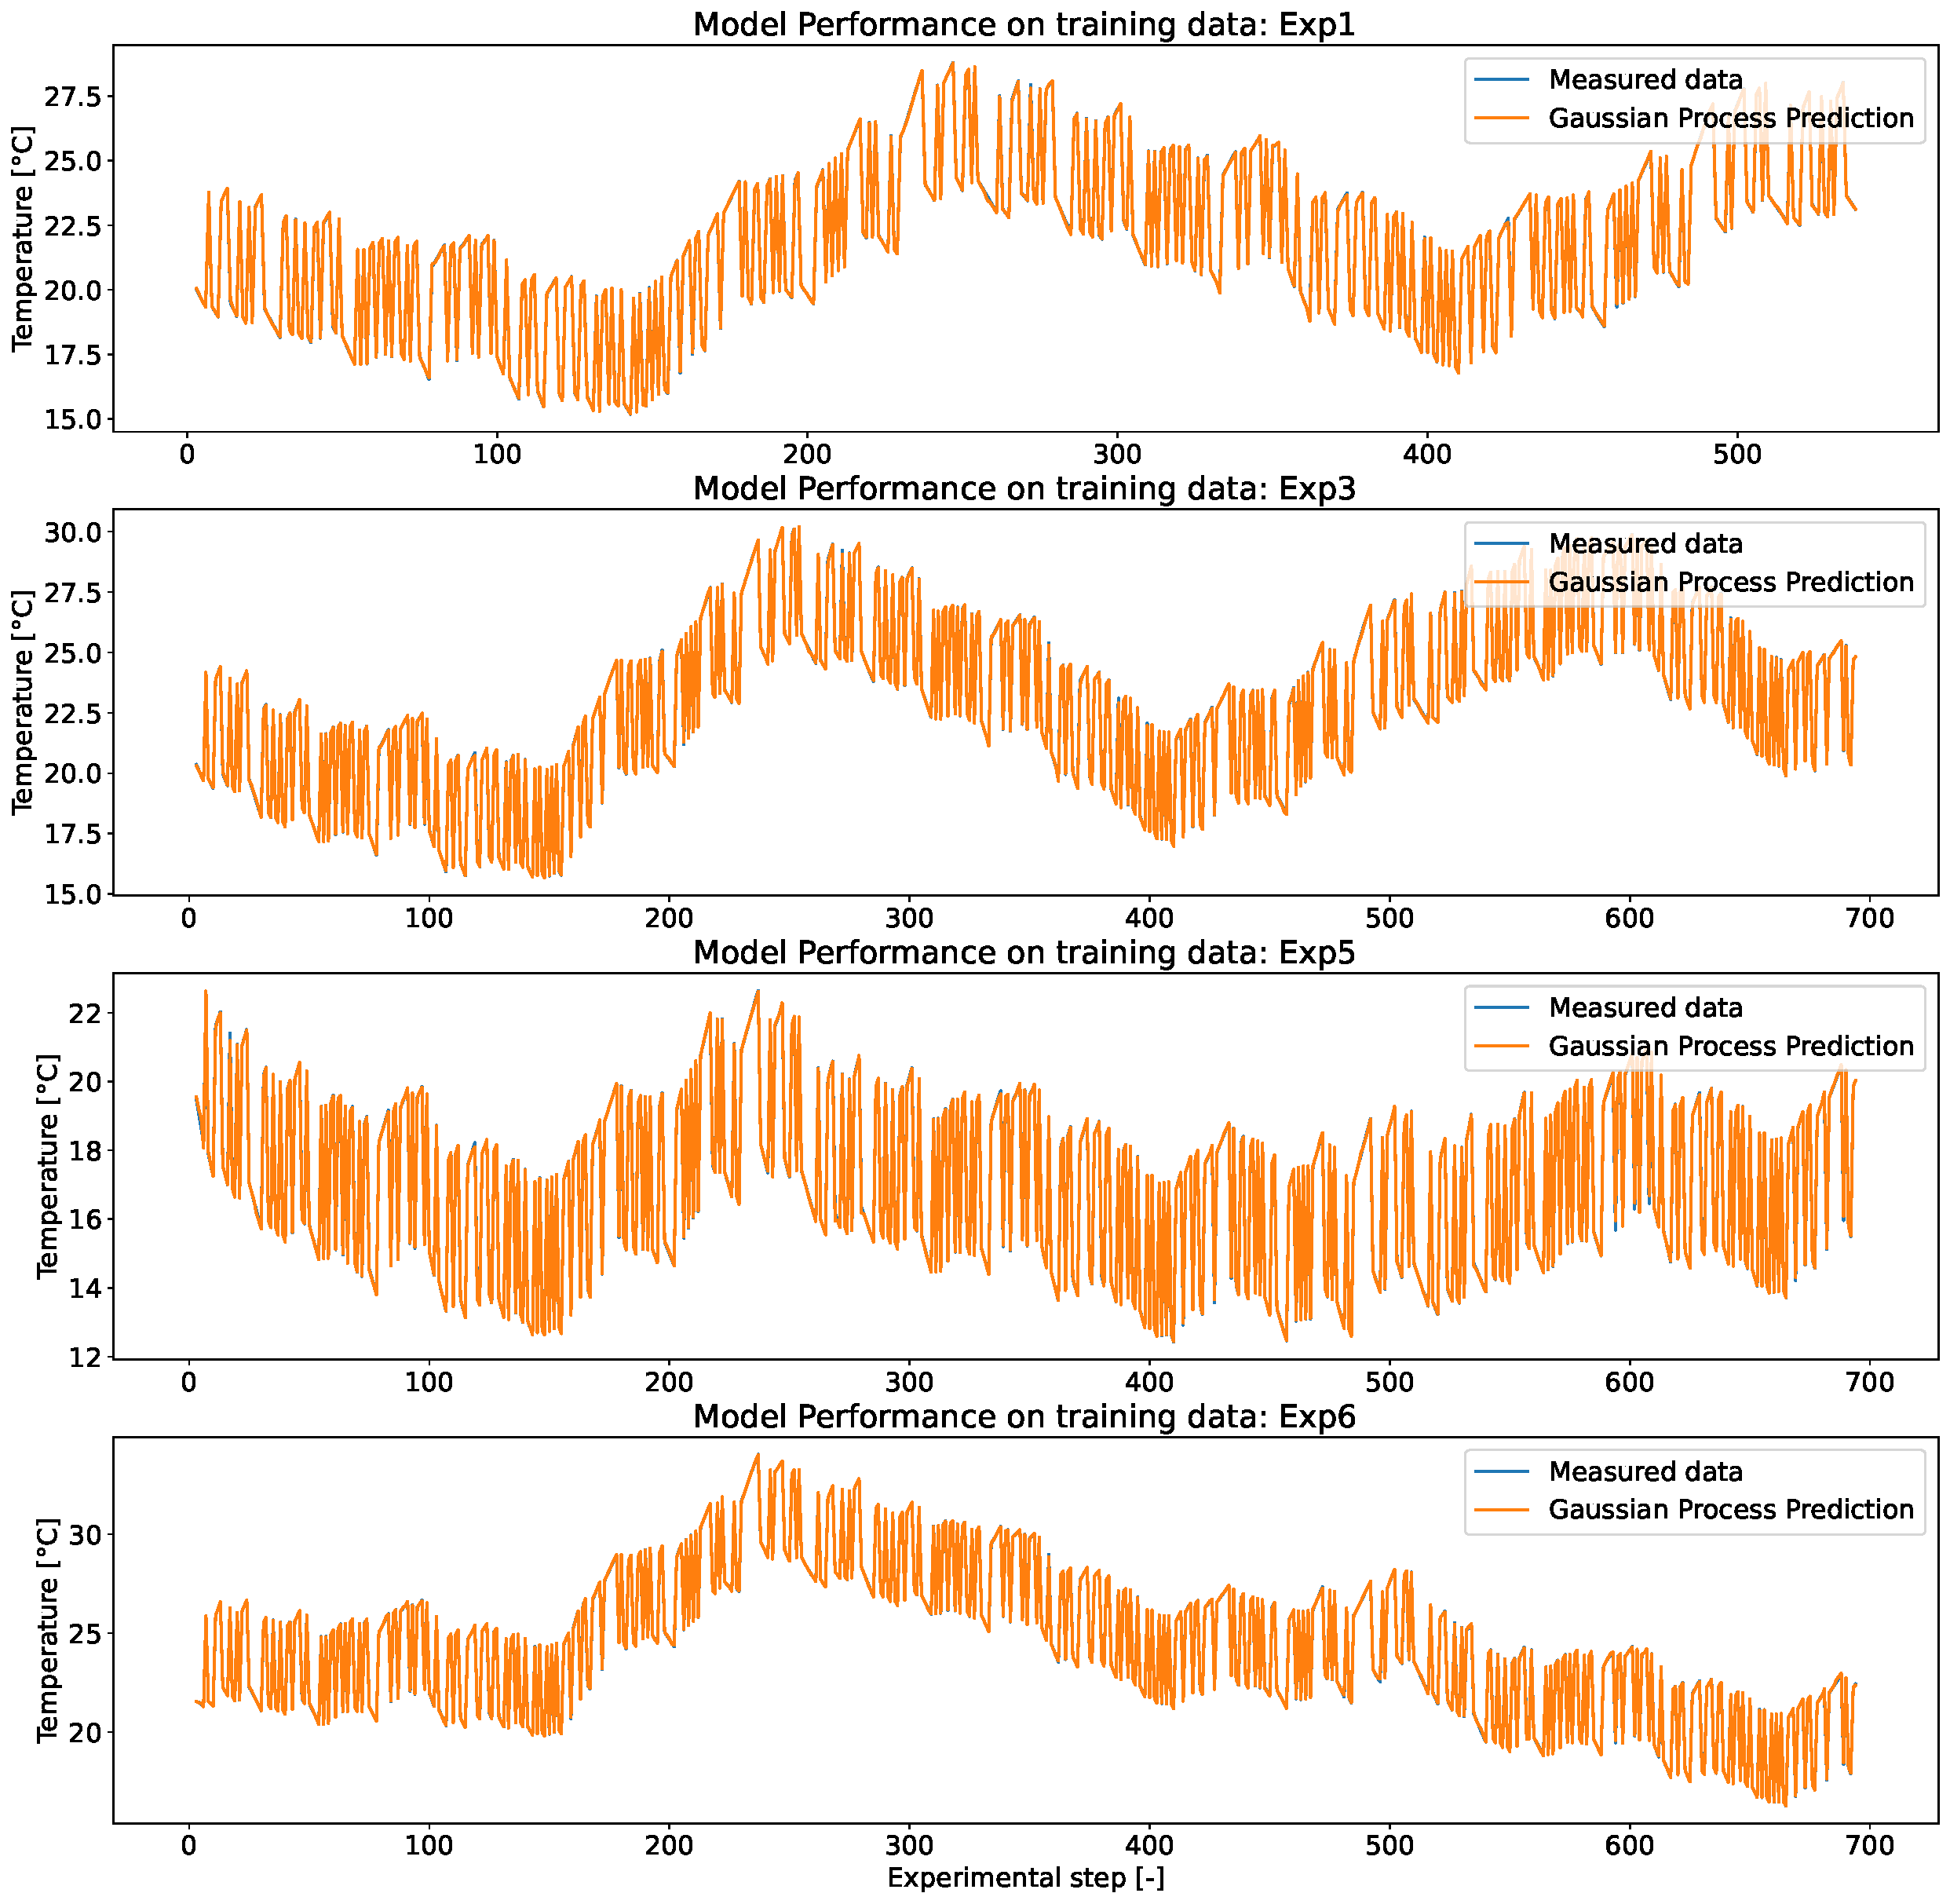
\includegraphics[width = \textwidth]{Plots/GP_113_training_performance.pdf}
    \caption{}
    \label{fig:GP_train_validation}
\end{figure}

\begin{figure}[ht]
    \centering
    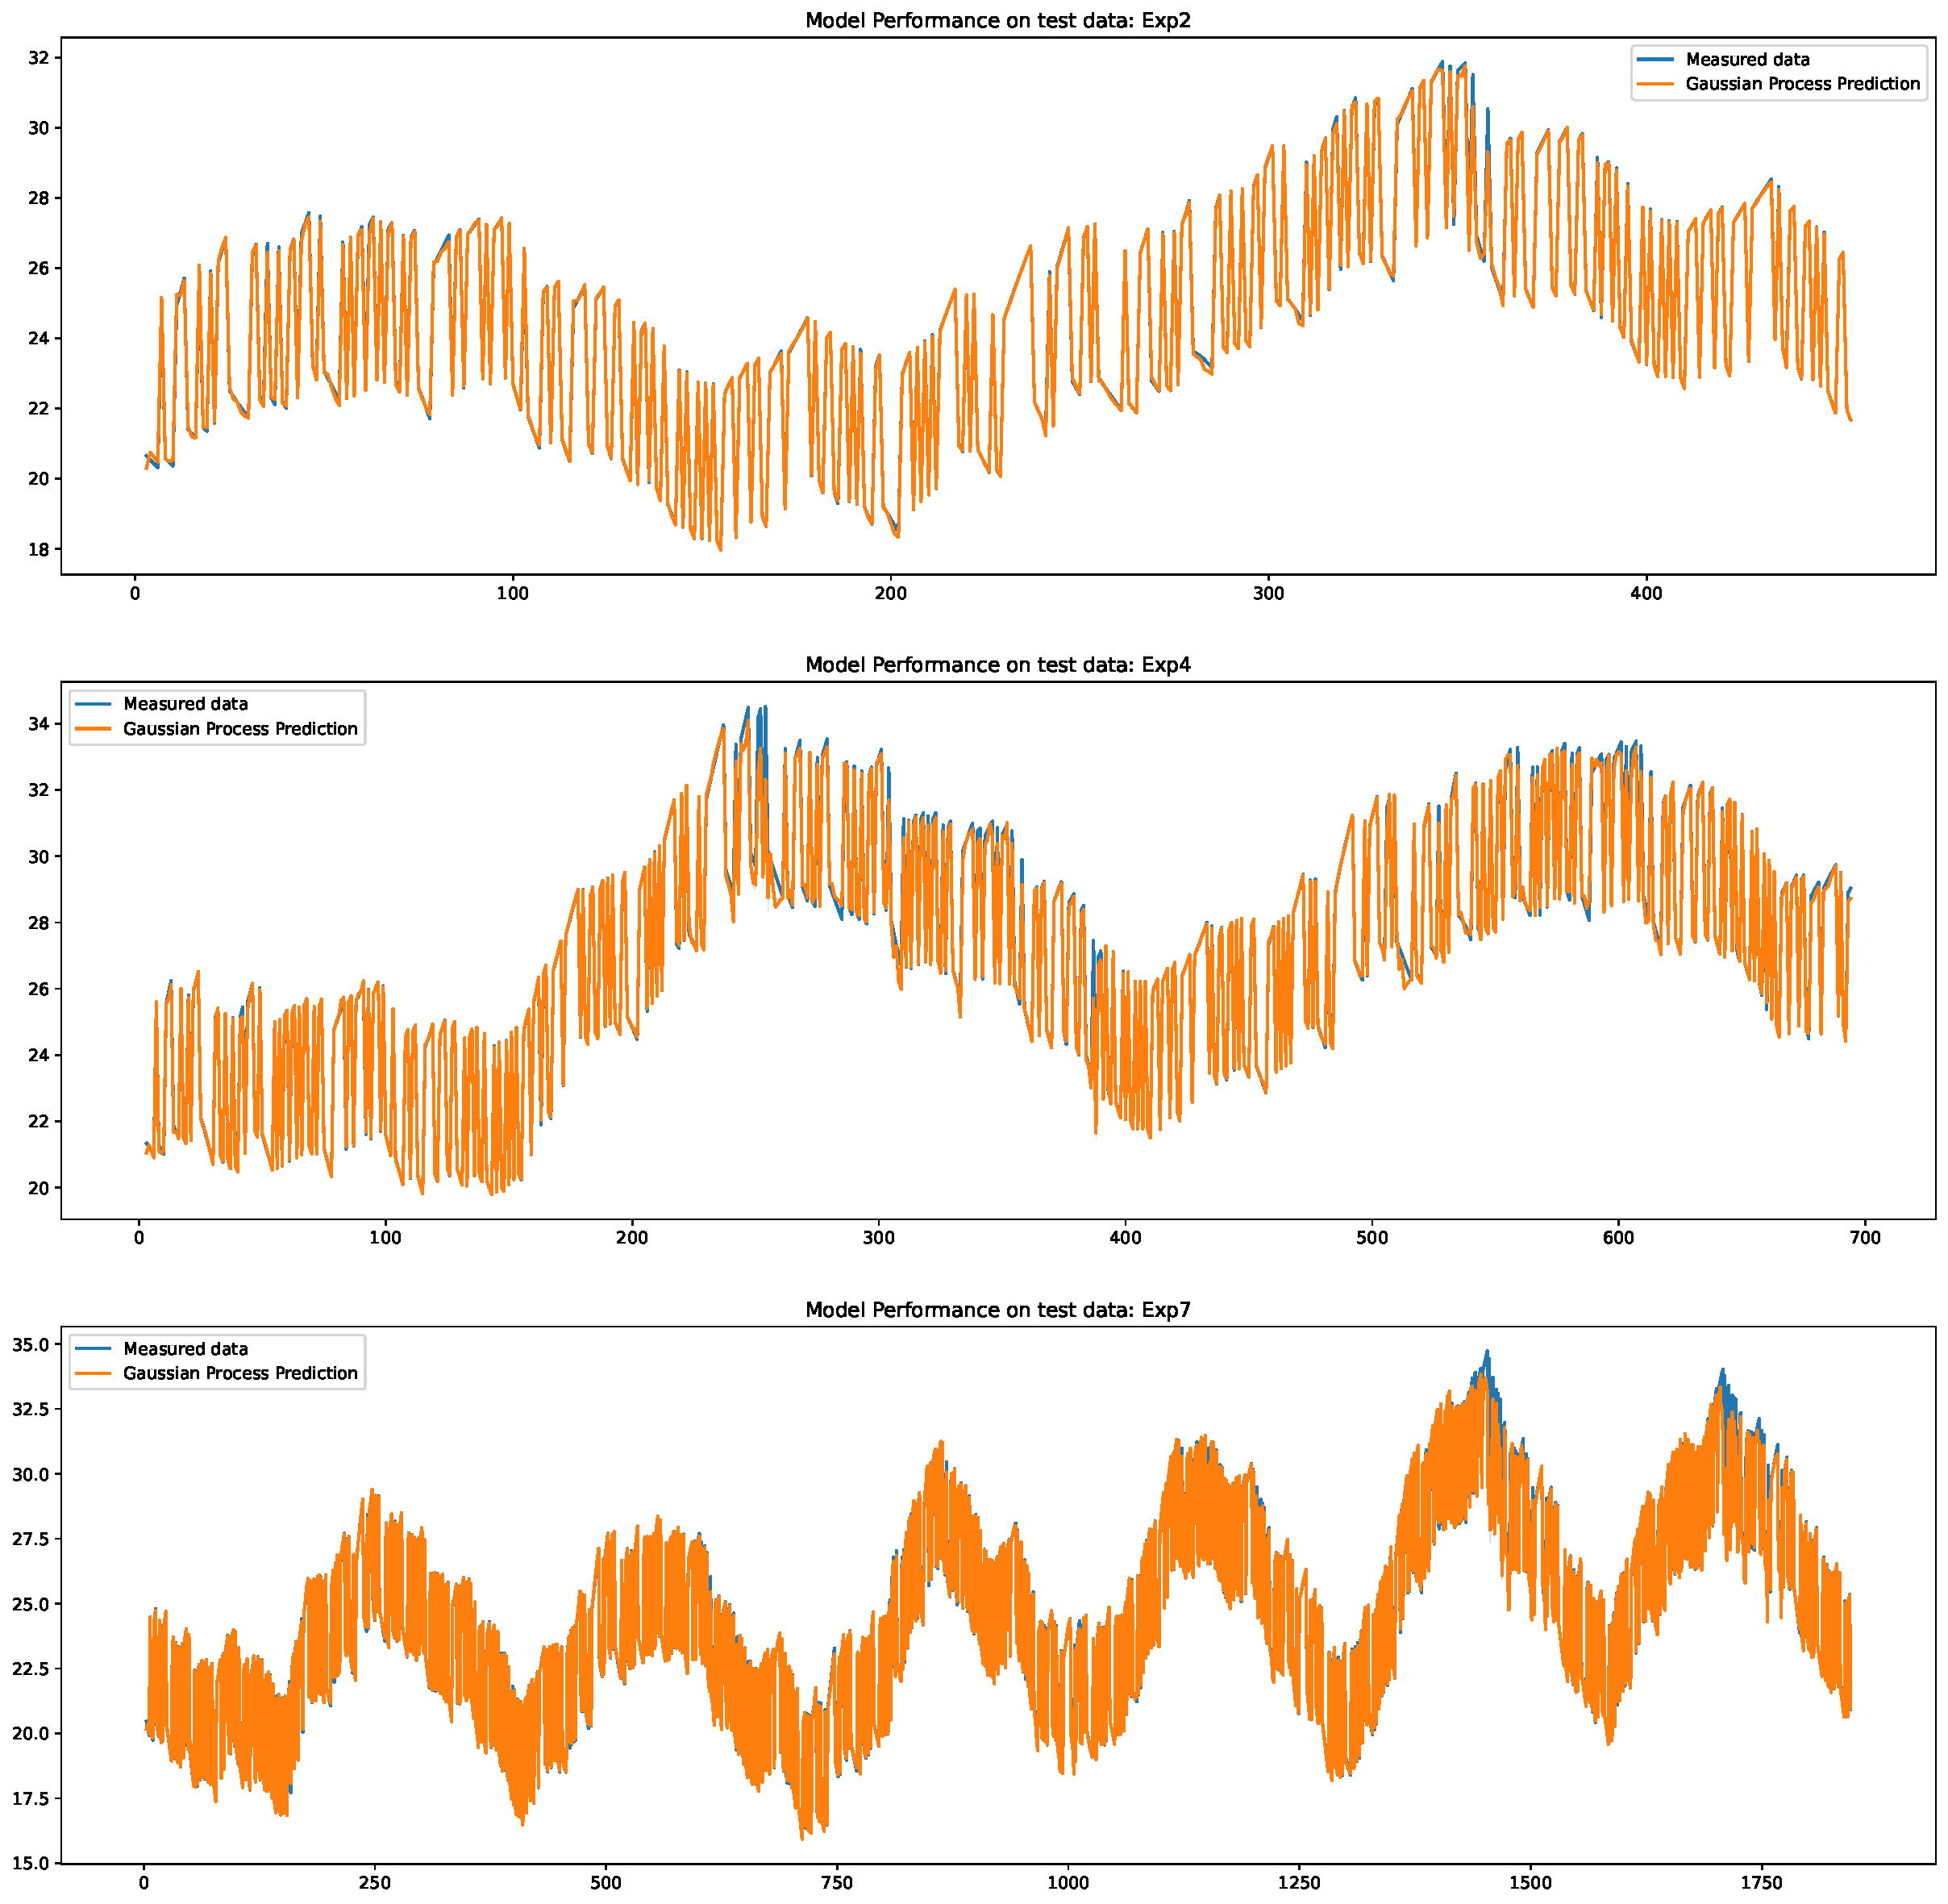
\includegraphics[width = \textwidth]{Plots/GP_113_test_performance.pdf}
    \caption{}
    \label{fig:GP_test_validation}
\end{figure}


\begin{figure}[ht]
    \centering
    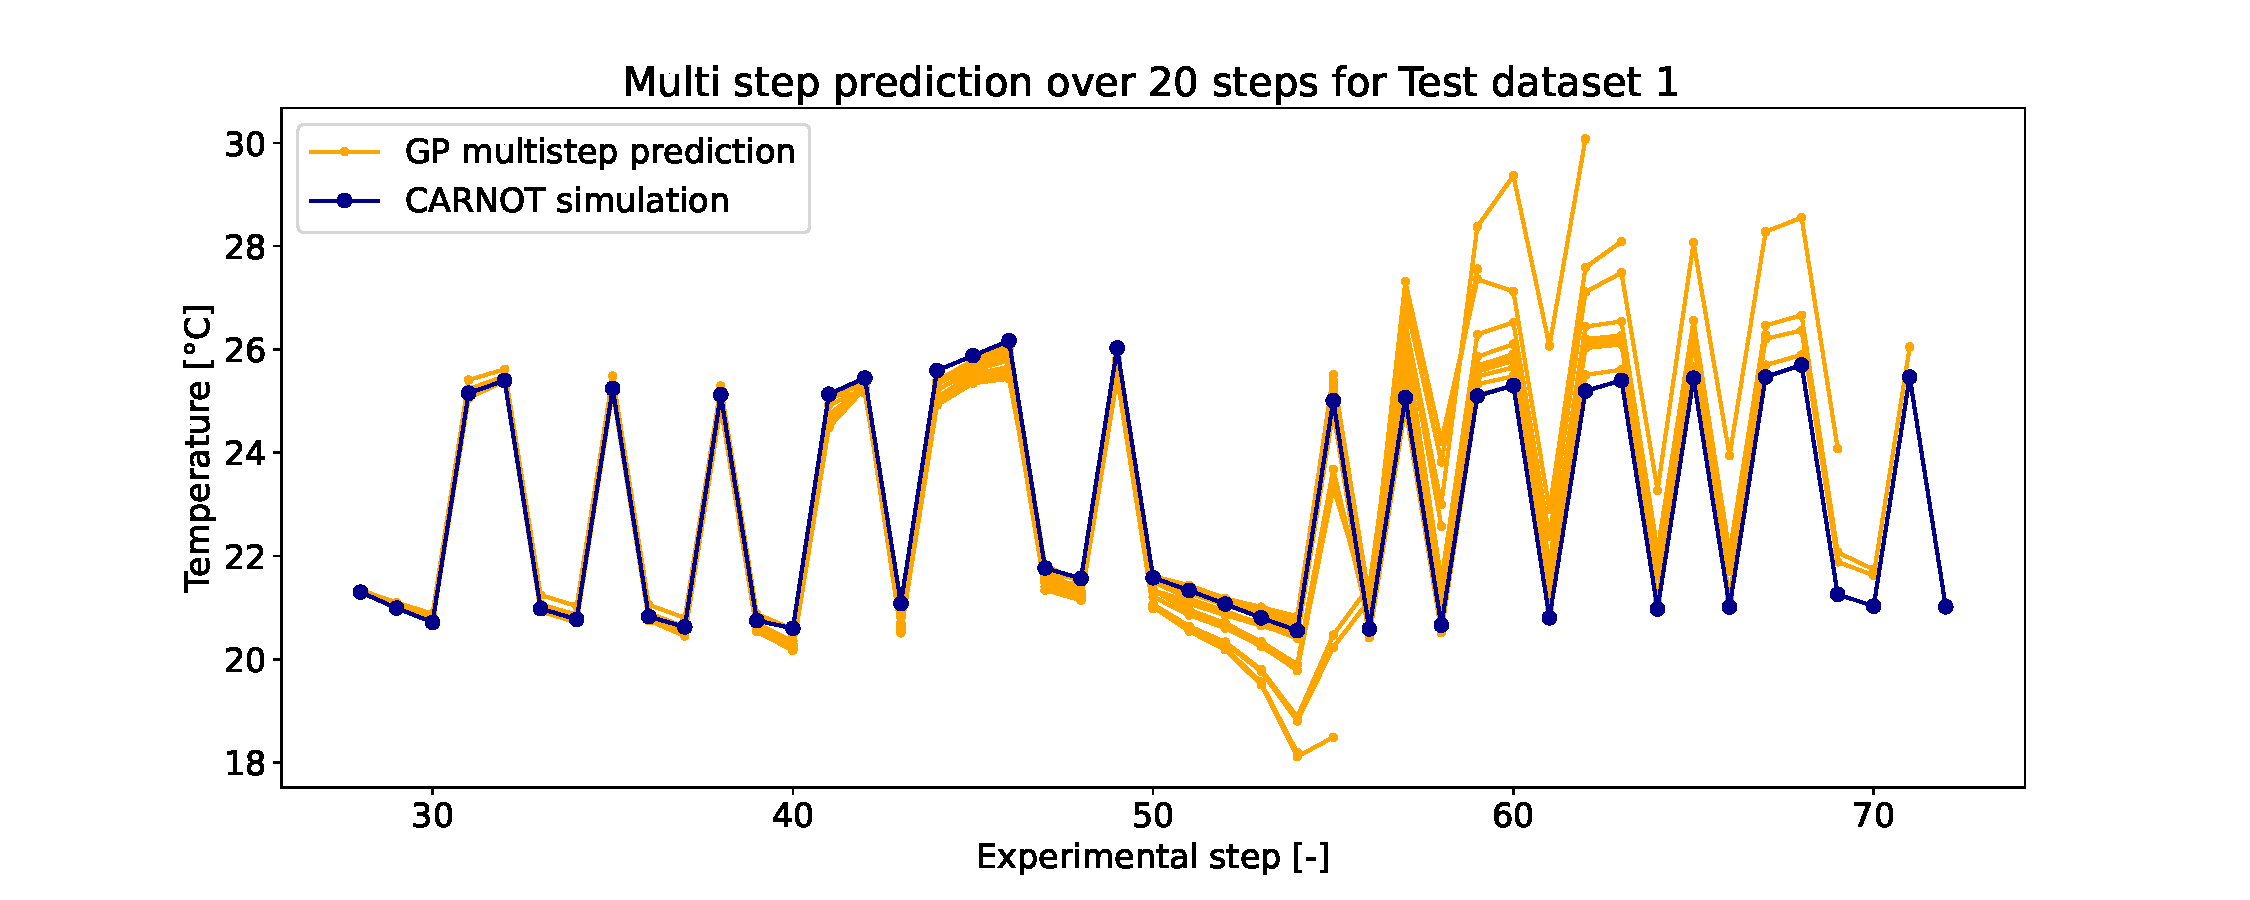
\includegraphics[width =
    \textwidth]{Plots/GP_113_-1pts_test_prediction_20_steps.pdf}
    \caption{}
    \label{fig:GP_multistep_validation}
\end{figure}

\clearpage

\subsubsection{Sparse and Variational Gaussian Process}

\begin{figure}[ht]
    \centering
    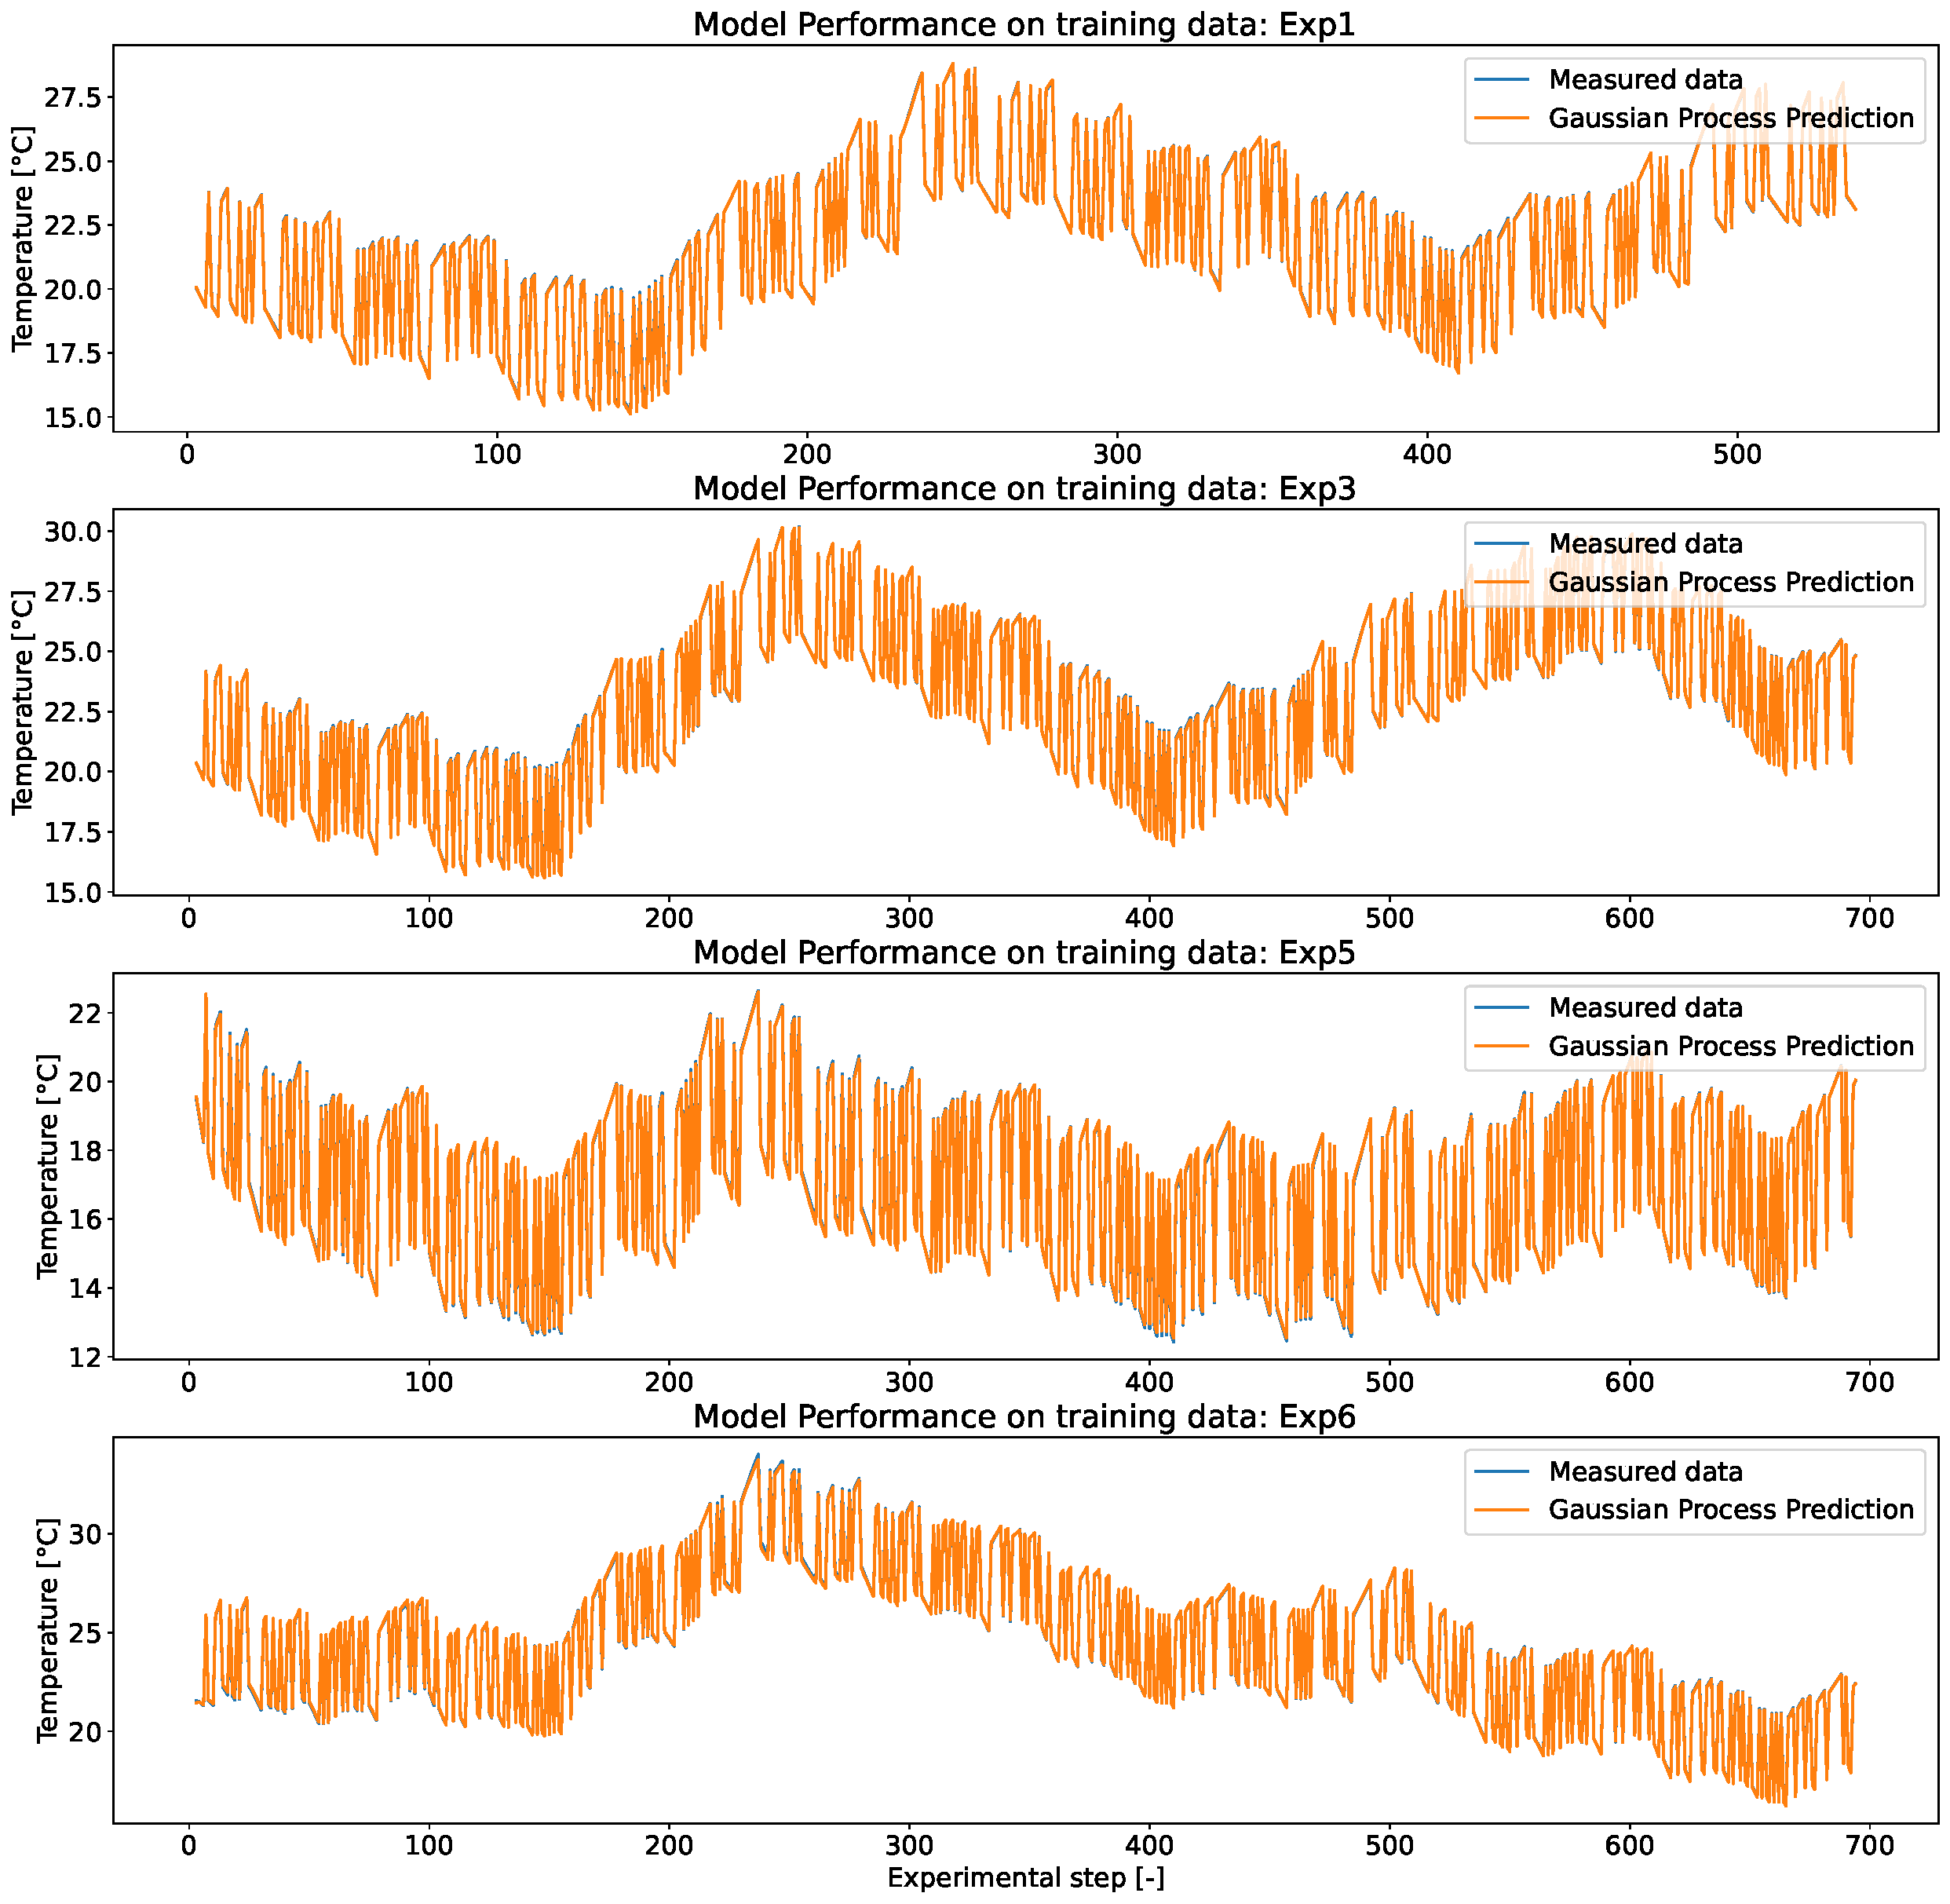
\includegraphics[width = \textwidth]{Plots/SVGP_123_training_performance.pdf}
    \caption{}
    \label{fig:SVGP_train_validation}
\end{figure}

\begin{figure}[ht]
    \centering
    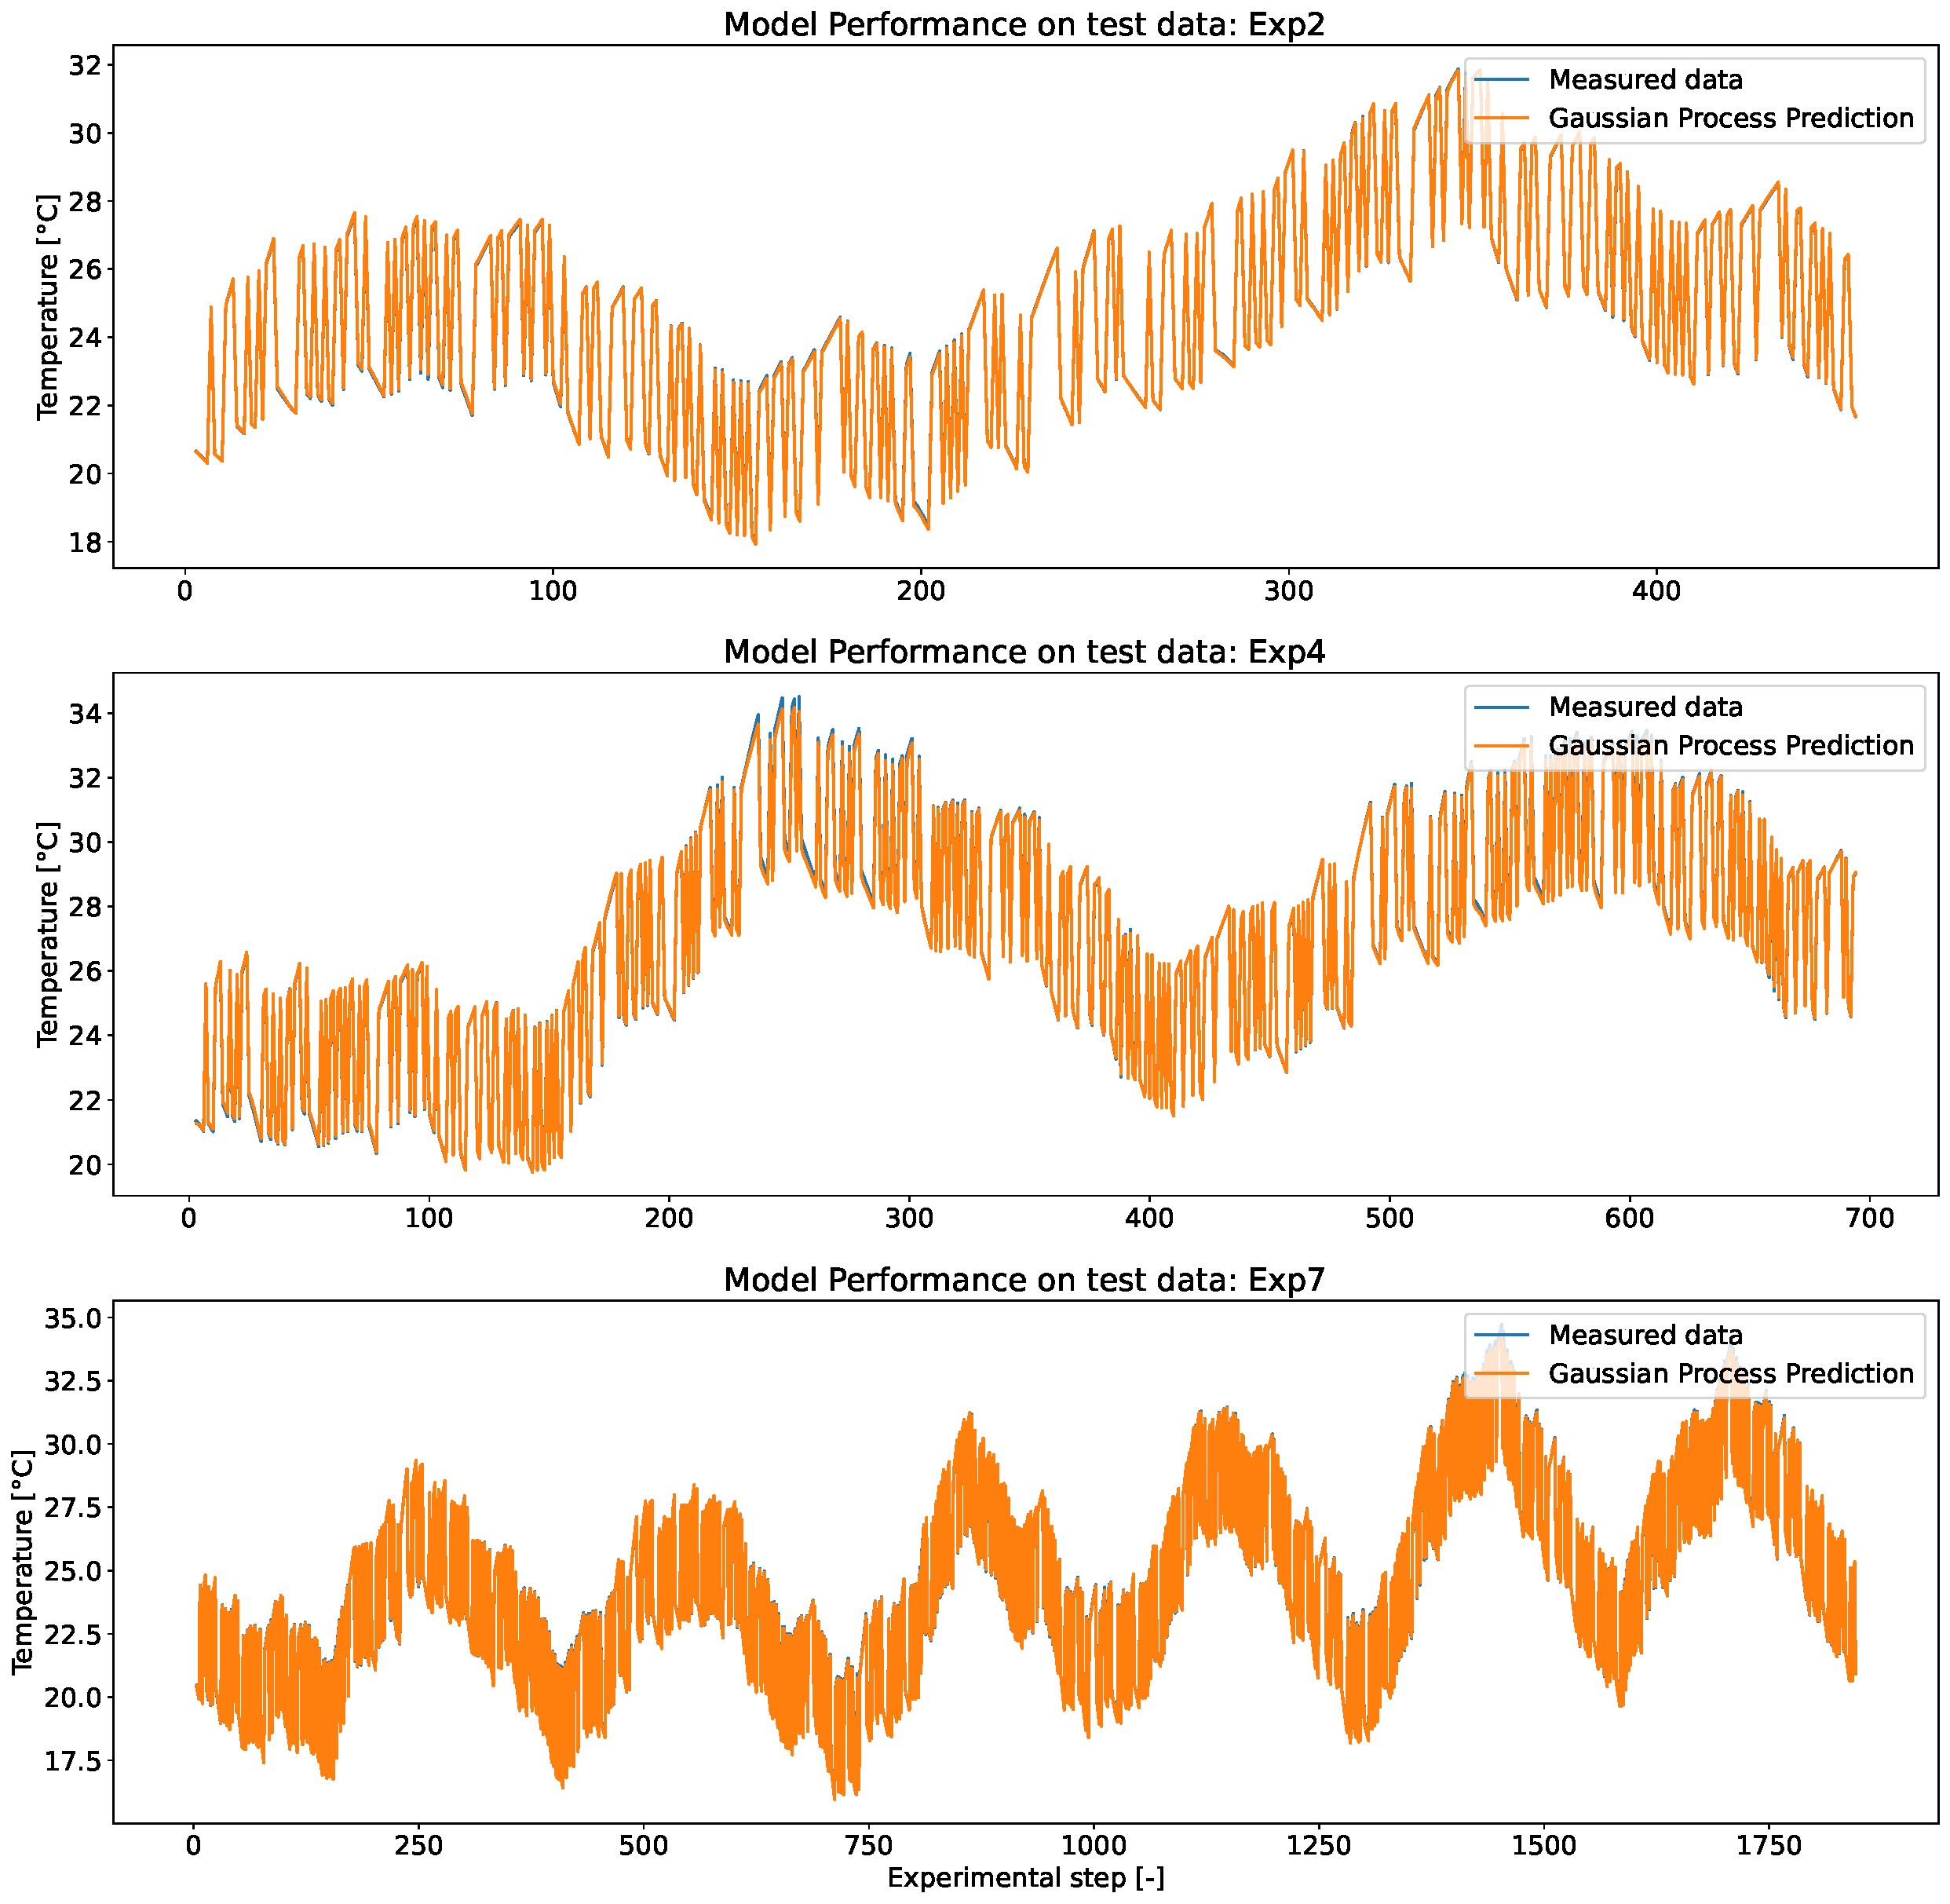
\includegraphics[width = \textwidth]{Plots/SVGP_123_test_performance.pdf}
    \caption{}
    \label{fig:SVGP_test_validation}
\end{figure}

\begin{figure}[ht]
    \centering
    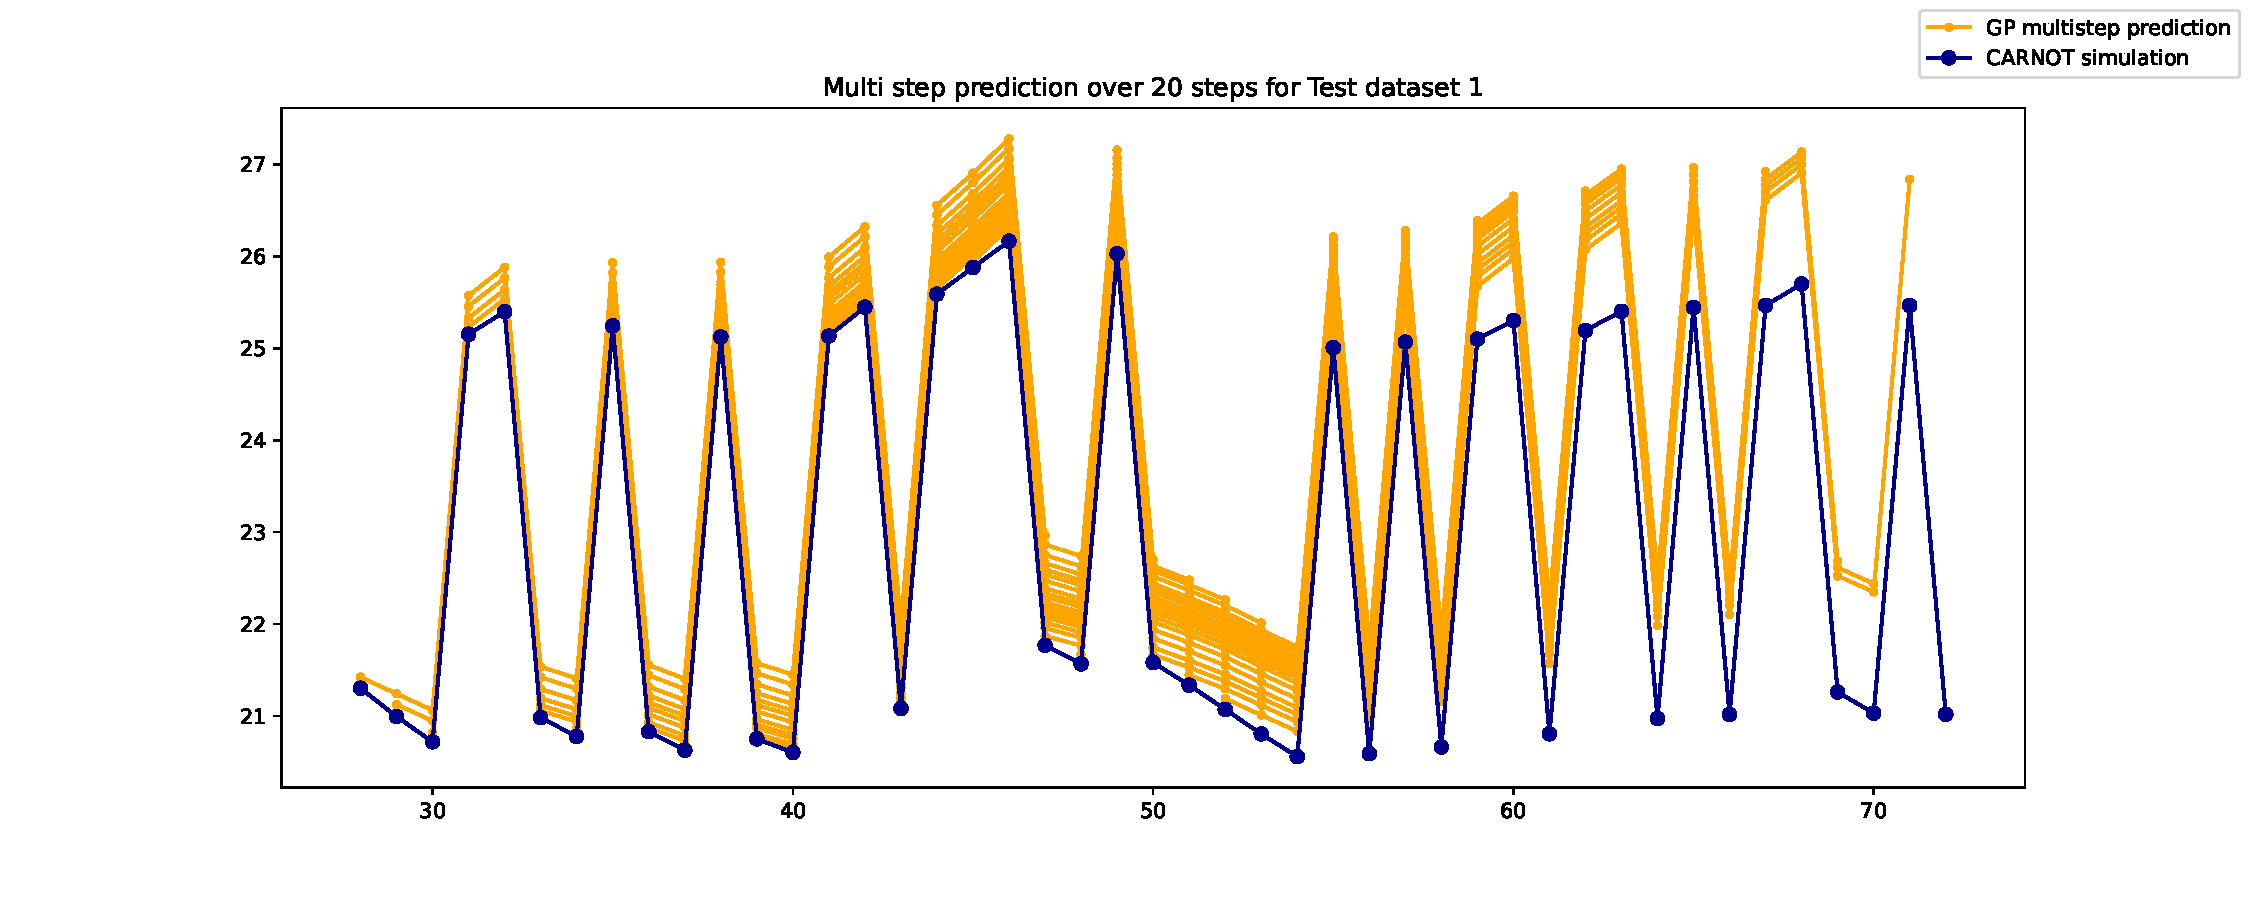
\includegraphics[width =
    \textwidth]{Plots/SVGP_123_test_prediction_20_steps.pdf}
    \caption{}
    \label{fig:SVGP_multistep_validation}
\end{figure}

\clearpage
